% Appendix

% Thomas, 2/2 -- feel free to delete this
\section{More category theory: properties of morphisms}

As we have seen, limits and colimits allow us ways to construct new objects, morphisms, and universal properties, over indexing diagrams. In particular we might be interested in relating certain properties of morphisms in a category to induced morphisms produced out of a colimit. As a motivating example, consider the following question.

\begin{question} Let $I$ be a small indexing diagram, and let $\alpha,\beta: I \to \Set$ denote two functors, and let $A_i := \alpha(i)$ and $B_i = \beta(i)$ denote the sets at each object $i\in I$. Suppose we have a natural transformation between these functors, consisting of functions $f_i \colon A_i \to B_i$ for each $i$. \textit{If each $f_i$ is injective, is it true that the induced map $f\colon \colim \alpha \to \colim \beta$ is injective as well?}
\end{question}

It turns out the answer to this diagram depends on the shape of $I$. It is true if the colimits are \textit{filtered}, which is a condition on the indexing diagram which tells us that it interacts well with finite limits. This motivates the more broad question of what properties of morphisms are preserved under limits and colimits. In general this is a hard question, but it will be important when we investigate fibrations and cofibrations in the category of topological spaces.


\subsection{Stability and closure definitions}



Let $\mathscr{C}$ be a category, not necessarily assumed to be locally small. We start with an easy definition.

\begin{definition}\label{def:closed-under-pullback} Let \textbf{P} be a property of morphisms in $\mathscr{C}$. We say that \textbf{P} is \textit{closed under composition} if, anytime we have two composable morphisms $f: x \to y$ and $g: y \to z$, if both $f$ and $g$ have property \textbf{P}, then the composite $g\circ f$ does as well.
\end{definition}


\begin{definition}\label{def:2-out-of-3} Let \textbf{P} be a property of morphisms in $\mathscr{C}$. We say that \textbf{P} \textit{satisfies 2-out-of-3} if for every commutative diagram of the form
\[ \begin{tikzcd}
    A\rar["f" above]\ar[dr,"g\circ f" below left] & B\dar["g" right]\\
     & C,\\
\end{tikzcd} \]
if any two of $f$, $g$, or $g\circ f$ have property \textbf{P}, then the third does as well.
\end{definition}


\begin{exercise} $\ $
\begin{enumerate}
    \item Prove that isomorphisms satisfy 2-out-of-3.
    \item In the category $\Set$, prove that injections and surjections do not satisfy 2-out-of-3.
\end{enumerate}
\end{exercise}

\begin{definition}\label{def:cancellative-properties} Let \textbf{P} be a property of morphisms.
\begin{enumerate}
    \item We say that \textbf{P} is a \textit{left cancellative property} if any time $g\circ f$ has property \textbf{P}, this implies that $f$ has property \textbf{P} as well.
    \item We say that \textbf{P} is a \textit{right cancellative property} if any time $g\circ f$ has property \textbf{P}, this implies that $g$ has property \textbf{P} as well.
\end{enumerate}
\end{definition}
As a warning to the reader, \textbf{the terminology in} \autoref{def:cancellative-properties} \textbf{is not standard}, although we would advocate for its usage. The notion of left cancellative properties is referred to as (CANC) in \cite[Appendix~C]{GortzWedhorn}, and has many examples in algebraic geometry (e.g. immersions, locally of finite type, purely inseparable, quasi-separated, separated). Many other examples occur under hypotheses on $g$, e.g. if it is separated or unramified. In a broader categorical context, we will see that mono-(resp. epi-)morphisms are left (resp. right) cancellative. 


\begin{definition}\label{def:closed-under-retracts} Let \textbf{P} be a property of morphisms. We say that \textbf{P} is \textit{closed under retracts} if, for any $f: A \to B$ with property \textbf{P}, and any $g: X \to Y$ fitting into a commutative diagram
\[ \begin{tikzcd}
    X\ar[rr,bend left=30,"\id_X" above]\dar["g" left]\rar & A\dar["f"]\rar & X\dar["g" right]\\
    Y\rar\ar[rr,bend right=30,"\id_Y" below] & B\rar & Y,
\end{tikzcd} \]
we have that $g$ has property \textbf{P} as well.
\end{definition}







\begin{definition} Let \textbf{P} be a property of morphisms. Then we say that \textbf{P} is \textit{stable under pullback} (often also called \textit{stable under base change}) if for any pullback diagram of the form
\[ \begin{tikzcd}
    C\rar["j" above]\dar["k" left]\pb & D\dar["f" right]\\
    A\rar["g" below] & B,\\
\end{tikzcd} \]
if $f$ has property \textbf{P}, then $k$ has property \textbf{P} as well. Dually, we say that \textbf{P} is \textit{stable under pushout} if for any pushout diagram of the form
\[ \begin{tikzcd}
    C\rar["j" above]\dar["k" left] & D\dar["f" right]\\
    A\rar["g" below] & B\po,\\
\end{tikzcd} \]
if $k$ has property \textbf{P}, then $f$ has property \textbf{P} as well.
\end{definition}

\begin{exercise}\label{exer:injective-stable-under-pullback} $\ $
\begin{enumerate}
    \item Prove that isomorphisms are always stable under pushout and pullback.
    \item Prove in the category $\Set$ that injective functions are stable under pullback, and surjective functions are stable under pushout.
\end{enumerate}
\end{exercise}


Thus far we have discussed closure properties internal to a category. We might wonder how properties translate across functors.

\begin{definition}\label{def:functor-preserve-reflect-properties} Let $F: \mathscr{C} \to \mathscr{D}$ be a functor, and let \textbf{P} be a property of morphisms.
\begin{enumerate}
    \item We say that $F$ \textit{preserves property} \textbf{P} if any time $f: x \to y$ is a morphisms in $\mathscr{C}$ with property \textbf{P}, we have that $Ff: Fx \to Fy$ has property \textbf{P} as well.

    \item We say that $F$ \textit{reflects property} \textbf{P} if any tie $f:x \to y$ is a morphism in $\mathscr{C}$, if $Ff: Fx \to Fy$ has property \textbf{P}, then $f$ must necessarily have property \textbf{P} as well.
\end{enumerate}
\end{definition}

\begin{remark} We have that $F$ always preserves isomorphisms (this is part of the property of being a functor). It is \textit{not true} that $F$ needs to reflect isomorphisms. For example if $X$ is a topological space with a non-trivial topology, then the map $\id : X \to X_{\text{disc}}$ from $X$ to itself with the discrete topology is not a homeomorphism, however its underlying set map is a bijection. (That is, the forgetful functor $\Top \to \Set$ does not reflect isomorphisms).
\end{remark}

\begin{exercise} If $F$ is full and faithful, it reflects isomorphisms.
\end{exercise}




\subsection{Monomorphisms and epimorphisms}

\autoref{exer:injective-stable-under-pullback} generalizes, as the notions of being injective and surjective in $\Set$ are equivalent to more abstract categorical conditions. We begin by generalizing injections.

\begin{definition}\label{def:monomorphism} Let $\mathscr{C}$ be a category. Then a morphism $f: x \to y$ is a \textit{monomorphism} if any of the following equivalent conditions hold:
\begin{enumerate}
    \item For any pair of morphisms $g,h : z \to x$ so that $f\circ g = f\circ h$, that is:
    \begin{align*}
        z \rightrightarrows x \to y,
    \end{align*}
    we have that $g = h$. (Another way of phrasing this is that $f$ is \textit{left cancellable}).

    \item The following diagram is a pullback:
\[ \begin{tikzcd}
    x\rar["\id_x" above]\dar["\id_x" left]\pb & x\dar["f" right]\\
    x\rar["f" below] & y.
\end{tikzcd} \]

If $\mathscr{C}$ is locally small, there is another equivalent condition:
\end{enumerate}


\begin{enumerate}
\setcounter{enumi}{2}
    \item The induced functor $\Hom_\mathscr{C}(-,x) \xto{f\circ -} \Hom_\mathscr{C}(-,y)$ is a natural injection, meaning that $\Hom_\mathscr{C}(z,x) \xto{f\circ -} \Hom_\mathscr{C}(z,y)$ is an injective function for any $z\in \mathscr{C}$.
\end{enumerate}
\end{definition}

\begin{exercise} Prove that the definitions in \autoref{def:monomorphism} are equivalent.
\end{exercise}

\begin{example} We have that isomorphisms and equalizers are always monomorphisms. Any morphism from a terminal object is a monomorphism.
\end{example}

\begin{exercise} \textit{(Closure properties of monomorphisms)}
\begin{enumerate}
    \item Monomorphisms are closed under composition
    \item Monomorphisms are stable under pullback
    \item Monomorphisms are left cancellative.
\end{enumerate}
\end{exercise}

\begin{exercise}\label{exer:left-adjoints-preserve-monomorphisms} \textit{(Left adjoints preserve monomorphisms)} Let $F: \mathscr{C} \rightleftarrows \mathscr{D} : G$ be an adjunction betweem locally small categories. Then if $f: x\to y$ is a monomorphism in $\mathscr{C}$, we have that $Ff : Fx \to Fy$ is a monomorphism in $\mathscr{D}$. (Hint: use the natural bijection associated to the adjunction, together with \autoref{def:monomorphism}, Definition (iii)).
\end{exercise}

There is a dual notion, called an \textit{epimorphism}.

\begin{definition}\label{def:epimorphism} Let $\mathscr{C}$ be a category. Then a morphism $f: x \to y$ is a \textit{epimorphism} if any of the following equivalent conditions hold:
\begin{enumerate}
    \item For any pair of morphisms $g,h : y \to z$ so that $g\circ f = h\circ f$, that is:
    \begin{align*}
         x \to y \rightrightarrows z,
    \end{align*}
    we have that $g = h$. (Another way of phrasing this is that $f$ is \textit{right cancellable}).

    \item The following diagram is a pushout:
\[ \begin{tikzcd}
    x\rar["f" above]\dar["f" left] & y\dar["\id_y" right]\\
    y\rar["\id_y" below] & y\po.
\end{tikzcd} \]

If $\mathscr{C}$ is locally small, there is another equivalent condition:
\end{enumerate}


\begin{enumerate}
\setcounter{enumi}{2}
    \item The induced functor $\Hom_\mathscr{C}(y,-) \xto{-\circ f} \Hom_\mathscr{C}(x,-)$ is a natural injection, meaning that $\Hom_\mathscr{C}(y,z) \xto{-\circ f} \Hom_\mathscr{C}(x,z)$ is an injective function for any $z\in \mathscr{C}$.
\end{enumerate}
\end{definition}

Epimorphisms satisfy all the dual properties to monomorphisms.

\begin{exercise}\label{exer:properties-of-epimorphisms} \textit{(Properties of epimorphisms)}
\begin{enumerate}
    \item Every isomorphism is an epimorphism, as is every coequalizer.
    \item Any morphism to an initial object is an epimorphism.
    \item Epimorphisms are closed under composition.
    \item Epimorphisms are stable under pushout.
    \item Epimorphisms are right cancellative. 
    \item Right adjoints preserve epimorphisms.
\end{enumerate}
\end{exercise}

As we have hinted at, monomorphisms and epimorphisms generalize the notions of injectivity and surjectivity in $\Set$. We can ask then whether categories which we think of as ``sets with extra data'' have the property that their monomorphisms are just those underlain by injections. Phrased differently, does the forgetful functor $U: \mathscr{C} \to \Set$ reflect mono and epimorphisms? This turns out to be true in some generality, but we must first make rigorous what it means to be a ``set with extra structure.''

\begin{definition}\label{def:concrete-category} A \textit{concrete category} is a locally small category $\mathscr{C}$, together with faithful functor to sets $U : \mathscr{C} \to \Set$. We think of this functor as ``forgetting'' the data.
\end{definition}

\begin{examples}\label{exs:concrete-categories} The following categories are concrete: $\Grp$, $\Poset$, $\Vect$, $\Top$, \todo{add more}.
\end{examples}


\begin{proposition} Any faithful functor reflects monomorphisms and epimorphisms.
\end{proposition}

Thus we see that all the categories in \autoref{exs:concrete-categories} have the property that their monomorphisms are underlying injections, and epimorphisms are underlying surjections. We summarize this in the following table.

\begin{table}[h]
    \centering
    \caption{Examples of monomorphisms and epimorphisms}
    \begin{tabular}{ p{2cm} l  p{5cm}  p{8cm} }
        \toprule
\textbf{Category}      
& \textbf{Monomorphisms}   
& \textbf{Epimorphisms} \\\midrule
$\Set$ & injections & surjections \\\hline

$\Grp$ & underlying injections & underlying surjections  \\\hline	 \bottomrule
    \end{tabular}
\end{table}


\begin{counterexample} We have that the inclusion $\Z \hookto \mathbb{Q}$ is an epimorphism in the category $\Ring$ of unital rings. This tells us that the forgetful functor $U: \Ring \to \Set$ is \textit{not} faithful.
\end{counterexample}

\subsection{Properties of morphisms can induce properties of objects}

Suppose we have a commutative diagram of the form
\[ \begin{tikzcd}
    A\rar["i" above]\ar[dr,"\id_A" below left] & B\dar["r" right]\\
     & A.
\end{tikzcd} \]
In this case we say the object $A$ is a \textit{retract} of $B$. We can ask about what properties of objects descend to their retracts, motivating the following definition.

\begin{definition}\label{def:property-objects-closed-under-retracts} Let \textbf{O} be a property of objects in $\mathscr{C}$ (we can just think of this as some subclass of the class of objects). Then we say that \textbf{O} is \textit{closed under retracts} if, any time $B \in \mathbf{O}$, and $A$ is a retract of $B$, we have that $A\in \mathbf{O}$ as well.
\end{definition}

We can ask about how a property of objects could potentially be related to a property of morphisms. In particular, we could ask about how properties of morphisms might induce properties of objects. Our perspective on this is stolen from algebraic geometry, in which a scheme is defined to have a property if and only if its structure morphism has the associated property. In the world of schemes and varieties, there basically don't exist properties for objects, only properties for morphisms. This is a feature of life with a terminal object. In many situations, such as topological spaces, we have the same luxury.

\begin{terminology}\label{term:inducing-properties-of-objects-from-properties-of-morphisms} Let $\mathscr{C}$ be a category with a terminal object $\ast$, and let \textbf{P} be a property of morphisms in $\mathscr{C}$. Then we have an \textit{induced property of objects} \textbf{O}, defined by saying that $X\in \mathbf{O}$ if the unique morphism $X \xto{!} \ast$ lies in \textbf{P}.
\end{terminology}

\begin{exercise} Let $\mathscr{C}$ be a category with a terminal object. Prove that if \textbf{P} is a property of morphisms closed under retracts in the sense of \autoref{def:closed-under-retracts}, then the induced property of objects is closed under retracts in the sense of \autoref{def:property-objects-closed-under-retracts}.
\end{exercise}

\begin{remark} The passage from fibrations to fibrant objects follows \autoref{term:inducing-properties-of-objects-from-properties-of-morphisms}.
\end{remark}






\subsection{Preservation properties under limits and colimits}

\begin{definition}\label{def:naturally-P} Let $I$ be an indexing category, let $\mathscr{C}$ be a category, and let \textbf{P} be a property of morphisms in $\mathscr{C}$. Let $f_1, f_2 : I \to \mathscr{C}$ be two diagrams in $\mathscr{C}$, and let $\eta: f_1 \Rightarrow f_2$ be a natural transformation between them. We say that $\eta$ \textit{has property} \textbf{P} \textit{levelwise} (or \textit{has property} \textbf{P} \textit{naturally}) if each of the components $\eta_c : f_1(c) \to f_2(c)$ has property \textbf{P}. As some examples:
\begin{enumerate}
    \item a \textit{natural isomorphism} is a natural transformation whose components are isomorphisms.
    \item a \textit{natural monomorphism} is a natural transformation whose components are monomorphisms.
\end{enumerate}
\end{definition}



\begin{definition}\label{def:colimit-preserve-property} Let $I$ be an indexing category, and let \textbf{P} be a property of morphisms in $\mathscr{C}$. We say that \textbf{P} \textit{is preserved under} $I$\textit{-shaped colimits} if, any time we have a natural transformation $\eta: f_1 \Rightarrow f_2$ which has property \textbf{P} levelwise, we have that the induced map
\begin{align*}
    \colim_I(f_1) \to \colim_I(f_2)
\end{align*}
is in \textbf{P} as well (assuming both colimits exist). Dually we have a notion of preservation under $I$-shaped limits.
\end{definition}

\begin{example} We have that isomorphisms are preserved under arbitrary limits and colimits.
\end{example}

\begin{example} If $I = \bullet\ \bullet$ is a discrete category on two points, we say that a property \textbf{P} is \textit{preserved under products} (resp. \textit{coproducts}) if it is preserved under $I$-shaped limits (resp. colimits).
\end{example}

\begin{proposition}\label{prop:monos-preserved-under-products} We have that
\begin{enumerate}
    \item Monomorphisms are preserved under products
    \item Epimorphisms are preserved under coproducts.
\end{enumerate}
\end{proposition}
\begin{proof} We will prove (1) and remark that (2) follows formally. Let $f: A \to B$ and $g: C \to D$ be monomorphisms. Then assuming their products exist, there is an induced map $(f \times g) : A \times C \to B \times D$. We claim that this is a monomorphism as well. Via \autoref{def:monomorphism}, we can restate the statement that $f$ and $g$ are monomorphisms into the statement that these diagrams are pullbacks
\[ \begin{tikzcd}
    A\rar\dar\pb & A\dar\\
    A\rar & B
\end{tikzcd} \quad\quad  \begin{tikzcd}
    C\rar\dar\pb & C\dar\\
    C\rar & D.
\end{tikzcd} \]
Since limits commute, we have that taking a product of the two pullbacks is the same as the pullback of the product of the two diagrams, that is, the following diagram is a pullback
\[ \begin{tikzcd}
    A \times C\rar["\id \times \id"]\dar["\id \times \id" left]\pb & A \times C\dar["f \times g" right]\\
    A \times C \rar["f \times g" below] & B \times D.
\end{tikzcd} \]
Thus $f \times g$ is a monomorphism.
\end{proof}


This is an instance of a more general phenomenon, namely functors preserving limits and colimits.

\begin{definition}\label{def:preserve-reflect-create-limits} Let $F:\mathscr{C} \to \mathscr{D}$ be a functor, and let $I$ be an indexing diagram.
\begin{enumerate}
    \item We say that $F$ \textit{preserves} $I$-shaped limits if, for any functor $j: I \to \mathscr{C}$, we have that the natural map is an isomorphism
    \begin{align*}
        F(\lim(j)) \cong \lim(F\circ j).
    \end{align*}
    That is, a limit cone over $j$ is sent to a limit cone over $F\circ j$.

    \item We say that $F$ \textit{reflects} $I$-shaped limits if, for any functor $j: I \to \mathscr{C}$, if we have that $F(c)$ is the limit of $F\circ j$, then $c$ is a limit of $j$. Phrased differently, a limit cone over $F\circ j$ in the image of $F$ must have come from a limit cone over $j$.

    \item We say $F$ \textit{creates} limits if it preserves and reflects them.
\end{enumerate}
We have analogous definitions for colimits.
\end{definition}

This relates to some things we have already seen: e.g. \autoref{prop:LAPC} said that left adjoints preserve colimits, and right adjoints preserve limits.

\begin{proposition}\label{prop:hom-functors-preserve-limits} Hom functors preserve limits in both arguments. That is, if $\mathscr{C}$ is a locally small category, then the bifunctor
\begin{align*}
    \Hom : \mathscr{C}^\op \times \mathscr{C} &\to \Set
\end{align*}
preserves limits in both arguments (limits in $\mathscr{C}^\op$ are colimits in $\mathscr{C}$).
\end{proposition}


\begin{corollary}\label{cor:Yoneda-embedding-preserves-limits} Let $\mathscr{C}$ be locally small. Then the Yoneda embedding $y: \mathscr{C} \hookto \Fun(\mathscr{C}^\op, \Set)$ preserves and reflects all limits.
\end{corollary}

\begin{proposition}\label{prop:fully-faithful-functor-reflects-limits-colimits} A fully faithful functor reflects all limits and colimits.
\end{proposition}


\begin{remark}\label{rmk:labelname} If $F$ is a functor preserving all limits over the diagram $I = \bullet \to \bullet \from \bullet$, we say that it \textit{preserves pullbacks}. Dually if $F$ preserves limits over the span diagram $J = \bullet \from \bullet \to \bullet$, we say it is \textit{preserves pushouts}.
\end{remark}

\begin{exercise}\label{exer:pullback-preserving-functor-preserves-monos} Let $F: \mathscr{C}\to \mathscr{D}$ be a functor.
\begin{enumerate}
    \item If $F$ preserves pullbacks, then it preserves monomorphisms.
    \item If $F$ preserves pushouts, then it preserves epimorphisms.
\end{enumerate}
\end{exercise}

Thus far we have defined two notions of preservation of properties. Namely, properties preserved under functors (as in \autoref{def:functor-preserve-reflect-properties}), and properties preserved under limits and colimits (as in \autoref{def:colimit-preserve-property}). We can see that these are both instances of the same idea.

\subsection{Colimits and limits as functors}

In order to relate these two notions of preservation, we should relate one to the other. In particular we claim that the most general notion of preservation of properties of morphisms is under a functor. In order to see that this encapsulates the other definition, we should view the construction of limits and colimits as a functor in some sense.

Let $\mathscr{C}$ be a category, and $I$ be an indexing category which we want to take limits and colimits over. Then there is a \textit{diagonal functor}
\begin{align*}
    \Delta : \mathscr{C} &\to \Fun(I, \mathscr{C}).
\end{align*}
This sends an object $c$ to the functor $\Delta_c: I \to \mathscr{C}$, where $\Delta_c(i) = c$ for all $i\in I$, and $\Delta_c(i \to i') = \id_c$. That is, $\Delta_c$ is really a constant functor at the object $c\in \mathscr{C}$. For a morphism $f:c\to c'$, we have an induced natural transformation  $\Delta_c \Rightarrow \Delta_{c'}$, all of whose components are $f$. 

\begin{exercise}\label{exer:diagonal-functor-into-functor-cat-fully-faithful} Show that $\Delta$ is fully faithful.
\end{exercise}


\begin{remark} We can consider the construction of colimits as a functor
\begin{align*}
    \colim : \Fun(I, \mathscr{C}) \to \mathscr{C},
\end{align*}
sending a diagram $I \to \mathscr{C}$ to the nadir of its colimit cone. Similarly $\lim: \Fun(I, \mathscr{C}) \to \mathscr{C}$ is a functor, sending a diagram to the apex of its limit cone.
\end{remark}

\begin{proposition} We have that $\colim \dashv \Delta \dashv \lim$ are adjoint functors.
\[ \begin{tikzcd}
    \mathscr{C}\rar["\Delta"] & \Fun(I,\mathscr{C})\lar[bend right=40,"\colim" above]\lar[bend left=40,"\lim" below].
\end{tikzcd} \]
\end{proposition}
\begin{proof} Let $c\in \mathscr{C}$, and let $j: I \to \mathscr{C}$ be a diagram. Then we have that $\Hom_{\Fun(I,\mathscr{C})}(\Delta_c, j)$ are the natural transformations of diagrams from $\Delta_c \to j$. That is, it is the \textit{set of cones over $j$ with vertex $c$}. By the universal property of the limit, for any such diagram, there is a unique map $c \to \lim(j)$, that is, we have a natural transformation
\begin{align*}
    \Hom_{\Fun(I,\mathscr{C})}(\Delta_c, j) \cong \Hom_\mathscr{C}(c, \lim(j)).
\end{align*}
A dual argument works to show that $\colim \dashv \Delta$.
\end{proof}

\begin{remark}\label{rmk:colimits-in-functor-categories} Since $\colim$ is a left adjoint, it now preserves colimits by \autoref{thm:LAPC}. We can ask what a colimit in $\Fun(I,\mathscr{C})$ looks like. Suppose we have a diagram of the form
\begin{align*}
    I \to \Fun(J, \mathscr{C}).
\end{align*}
This corresponds under adjunction to a map $I \times J \to \Fun(\mathscr{C})$. We can ask whether
\begin{align*}
    \colim \left( I \to \Fun(J, \mathscr{C}) \right) \overset{?}{=} \colim \left( I \times J \to \mathscr{C} \right).
\end{align*}
If $I$ and $J$ are small indexing diagrams, and $\mathscr{C}$ has all colimits, this is certainly true {\color{blue} because Kan extensions are computed pointwise in this context --- find a better way to explain this though}.
\end{remark}


\begin{theorem}\label{thm:colimits-commute} \textit{(Colimits commute)} Let $I$ and $J$ be small indexing diagrams, and let $\mathscr{C}$ be cocomplete (or at least have all the colimits we are discussing here exist). Then for any bifunctor
\begin{align*}
    F: I \times J \to \mathscr{C}
\end{align*}
we have a canonical isomorphism
\begin{align*}
    \lim_i \lim_j F(i,j) \cong \lim_j \lim_i F(i,j).
\end{align*}
See for example \cite[3.8.1]{Riehl-context}. A dual statement is true for colimits as well.
\end{theorem}





\begin{center}
    [[todo]]    
\end{center}

\subsection{Filtered limits and colimits}

In \autoref{thm:colimits-commute}, we could replace one of the limits with a colimit and ask if everything is still true. Phrased differently, if we have a functor $F: I \times J \to \mathscr{C}$, we can compare
\begin{align*}
    \colim_j \lim_i F(i,j) \text{ and } \lim_i \colim_j F(i,j).
\end{align*}
We first show that there definitely exists a map between them.

\begin{proposition}\label{prop:labelname} There is a canonical map
\begin{align*}
    \colim_j \lim_i F(i,j) \to \lim_i \colim_j F(i,j).
\end{align*}
\end{proposition}

\begin{proof} By \autoref{exer:diagonal-functor-into-functor-cat-fully-faithful}, we have that $\Delta$ is fully faithful, therefore the unit and counit maps are natural isomorphisms:
\begin{align*}
    1_{\Fun(I,\mathscr{C})} \xto{\sim} \lim \circ \Delta \\
    \colim \circ \Delta \xto{\sim}  1_\mathscr{C}.
\end{align*}
Now consider the diagram
\[ \begin{tikzcd}
    \Fun(I \times J, \mathscr{C})\rar[bend left=30,"\colim_I" above]\rar[bend right=30,"\lim_I" below] & \Fun(J, \mathscr{C})\lar["\Delta"]\rar[bend left=30,"\colim_J" above]\rar[bend right=30,"\lim_J" below] & \mathscr{C}\lar["\Delta"].\\
\end{tikzcd} \]

The composite $\colim_J \lim_I$ weaves through the middle of this diagram in a wave shape. By looping through the units of adjunctions, we have a map

Therefore we see that
\begin{align*}
    \colim_J \lim_I = 1 \colim_J \lim_I 1 \to \left( \lim_J \Delta \right)\colim_J \lim_I \left( \Delta \colim_I \right) \\
    &= 
\end{align*}
For an explicit computation of this map, see \cite[3.8.3]{Riehl-context}.
\end{proof}



\begin{center}
    [[todo]]    
\end{center}




\section{Unsorted subsections on category theory}

\subsection{Conventions}

We record some standard notation for use in these notes.

\begin{notation}\label{nota:initial-terminal-objects} We denote an \textit{initial object} in a category $\mathscr{C}$ by $\emptyset$. We denote a \textit{terminal object} in a category $\mathscr{C}$ by $\ast$. If $X \in \mathscr{C}$ is arbitrary, it receives a unique map from the initial object and to the terminal object. We decorate each of these with a shriek:
\begin{align*}
    \emptyset &\xto{!} X \\
    X &\xto{!} \ast.
\end{align*}
\end{notation}

\begin{notation}\label{nota:diagonal-map} Let $\mathscr{C}$ be a category, and let $X\in \mathscr{C}$ be an arbitrary object. If the product $X \times X$ exists, there is a \textit{diagonal map}, which we denote by
\begin{align*}
    X \xto{\Delta} X \times X,
\end{align*}
defined to be the unique map provided to us by the universal property of the product
\[ \begin{tikzcd}
     & X\dar\ar[ddl,bend right=10,"\id_X" left]\ar[ddr,bend left=10,"\id_X" right]\dar[dashed,"\Delta" right] & \\
     & X \times X\ar[dl,"\pr_1" below right]\ar[dr,"\pr_2" below left] & \\
    X &  & X.
\end{tikzcd} \]
\end{notation}
\begin{notation}\label{nota:fold-map} Let $\mathscr{C}$ be a category, and let $X\in \mathscr{C}$ be an arbitrary object. If the coproduct $X \amalg X$, there is a \textit{fold map}, which we denote by
\begin{align*}
    X \amalg X \xto{\nabla} X,
\end{align*}
defined to be the unique map provided to us by the universal property of the coproduct
\[ \begin{tikzcd}
    X\ar[dr,"i_1" above right]\ar[ddr,bend right=10,"\id_X" left] &  & X\ar[dl,"i_2" above left]\ar[ddl,bend left=10,"\id_X" right]\\
     & X \amalg X\dar[dashed,"\nabla" right]& \\
     & X. & \\
\end{tikzcd} \]
\end{notation}

The terminology for the \textit{diagonal} map comes from the world of sets (or concrete categories more generally), where the function $\Delta: X \to X \times X$ is defined elementwise by $x \mapsto (x,x)$. That is, its image is the diagonal in the product. The \textit{fold} map comes from the mental image of taking two disjoint copies of $X$ and folding them over one another into one copy of $X$.

\begin{notation}\label{nota:product-coproduct-of-morphisms} Let $\mathscr{C}$ be a category with products, and let $f: A \to B$ and $g: C \to D$ be two morphisms. Then we denote by
\begin{align*}
    f \times g : A \times C \to B \times D
\end{align*}
the morphism given via the universal property
\[ \begin{tikzcd}
     & A \times B\ar[dl]\ar[dr]\dar[dashed,"f \times g"] & \\
    A\dar["f" left] & C \times D\ar[dl]\ar[dr] & B\dar["g" right]\\
    C &  & D.
\end{tikzcd} \]
Similarly if $\mathscr{C}$ is a category with coproducts, we denote by
\begin{align*}
    f \amalg g : A \amalg C \to B \amalg D
\end{align*}
the morphism provided by the universal property
\[ \begin{tikzcd}
    A\ar[dr]\dar["f" left] &  & B\ar[dl]\dar["g" right]\\
    C\ar[dr] & A\amalg B\dar[dashed,"f \amalg g"] & D\ar[dl]\\
     & C \amalg D. &
\end{tikzcd} \]

\end{notation}




\subsection{Laws for pullbacks and pushouts}

Frequently we will be asked to glue together commutative squares and talk about whether the composite square is a pullback and/or whether the individual squares are pullbacks. This is discussed in the so-called \textit{pasting law}.

\begin{proposition}\label{prop:pasting-law-pullbacks-pushouts} \textit{(Pasting law for pullbacks and pushouts)} Let $\mathscr{C}$ be an arbitrary category, and consider a commutative diagram of the following form
\[ \begin{tikzcd}
    \bullet\rar\dar & \bullet\rar\dar & \bullet\dar\\
    \bullet\rar & \bullet\rar & \bullet.
\end{tikzcd} \]
\begin{enumerate}
    \item If the right square is a pullback, then the total square is a pullback if and only if the left square is a pullback.
    \item If the left square is a pushout, then the total square is a pushout if and only if the right square is a pushout.
\end{enumerate}
\end{proposition}

We also have the ``magic square,'' which is generally stated for varieties or schemes, but holds in a more broad context.

\begin{proposition}\label{prop:magic-pullback-square} \textit{(Magic pullback square)} Let $\mathscr{C}$ be a locally small category with products and pullbacks. Let $f: X \to Z$, and $g: Y \to Z$ be morphisms in $\mathscr{C}$. Then the following square is a pullback
\[ \begin{tikzcd}
    X \times_Y Z\rar\dar\pb & X \times Y\dar["f \times g" right]\\
    Z\rar["\Delta" below] & Z \times Z.
\end{tikzcd} \]
\end{proposition}
\begin{proof} We first check that this holds if $\mathscr{C} = \Set$. This is certainly true, since elements of $(X \times Y)\times_{Z \times Z} Z$ are precisely elements $(x,y) \in X \times Y$ so that $f(x) = g(y)$. Then for any locally small category $\mathscr{C}$, we have that this diagram is a levelwise pullback in $\Fun \left( \mathscr{C}^\op, \Set \right)$. Finally we remark that under the Yoneda embedding $y : \mathscr{C} \hookto \Fun(\mathscr{C}^\op, \Set)$, limits are reflected.
\end{proof}

The magic pullback square is generally stated in the following form.

\begin{corollary}\label{cor:magic-square-over-S} Let $\mathscr{C}$ be a locally small category, and $S\in \mathscr{C}$ be any element. Then if $f: X \to Z$ and $g : Y \to Z$ are morphisms over $S$, we have a pullback square
\[ \begin{tikzcd}
    X \times_Y Z\rar\dar\pb & X \times_S Y\dar["f \times g"]\\
    Z\rar["\Delta" below] & Z \times_S Z.
\end{tikzcd} \]
\end{corollary}


\section{Homotopy colimits}

Here we explore instances in which homotopy (co)limits appear in the basic curriculum of algebraic topology, namely in \cite{Hatcher} and \cite{May}. A rigorous treatment of homotopy colimits is not provided here, we defer to the far better expositors Dugger and Riehl for their expositions of simplicial and categorical understandings of homotopy colimits \cite{Dugger,Riehl-hocolims}. We would posit that homotopy colimits are an intuitive concept to grasp and work with, and that recognizing them as they occur in basic algebraic topology provides the reader with another tool to grasp the material.

\subsection{Intro to homotopy colimits}

As described above, we neglect to provide a rigorous definition of homotopy colimits, as the rigorous definitions ($\hocolim$ is the derived functor of $\colim$; homotopy colimits are the geometric realization of the simplicial replacement) are technical to state. Instead, we provide the following characterization of homotopy colimits, based on an intuitive understanding of colimits:
\begin{center}
    Colimits are obtained by gluing spaces.\\
    \textit{Homotopy colimits} are obtained by gluing spaces \textit{with wiggle room, in a continuous fashion}.
\end{center}

What do we mean by this? Say we want to glue two spaces $X$ and $Y$ together along distinguished basepoints to form a wedge product $X \vee Y$. How do we do this in general? We take the disjoint union $X \amalg Y$ and mod out by the equivalence relation $x_0 \sim y_0$. Phrased differently, we glue $x_0$ and $y_0$ together to force them to become the same point in the quotient space.

Instead of gluing them directly together, we could instead draw a path connecting $x_0$ and $y_0$. Now instead of formally identifying the two points, we provide them a path by which one can travel to the other.

\begin{figure}[H]
  \scalebox{0.2}{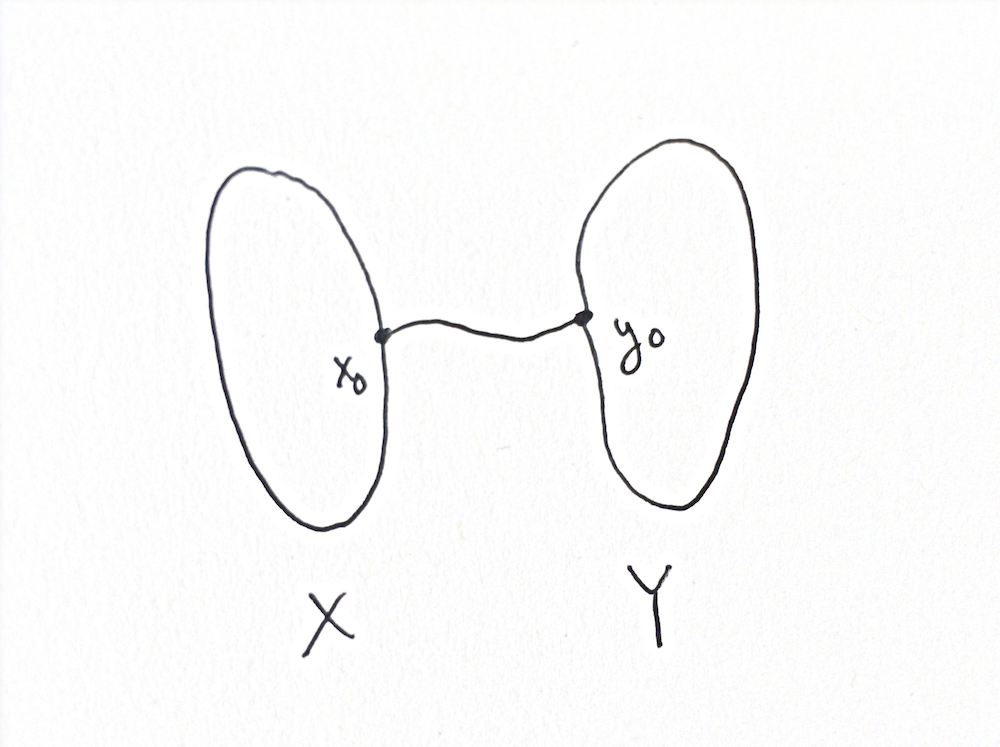
\includegraphics{pics/whisker-gluing.png}}
  \centering
\end{figure}




\begin{example} As another example, suppose $\ast \hookto X$ is the inclusion of a point $x\in X$. Taking the cofiber of this map\footnote{Recall the cofiber of a map $f: X \to Y$ is the colimit $\colim \left( \ast \from X \xto{f} Y \right)$.} is the same as simply gluing the point $\ast$ to $x\in X$, and you simply end up with the space $X$. If, instead, you wanted to take the \textit{homotopy cofiber} of this map, you would end up with the space $X$, with a small whisker protruding from the point $x$, ending at the point $\ast$. This procedure has a name, and it is actually called \textit{whiskering}. For example if $(X,x)$ is a based space which is not well based\footnote{Recall a space is \textit{well-based/non-degenerately based} if the inclusion of the basepoint is a cofibraion.}, we can take the based space $(\hocolim(\ast \hookto X),\ast)$, which becomes well-based.
\end{example}

\begin{figure}[H]
  \scalebox{0.2}{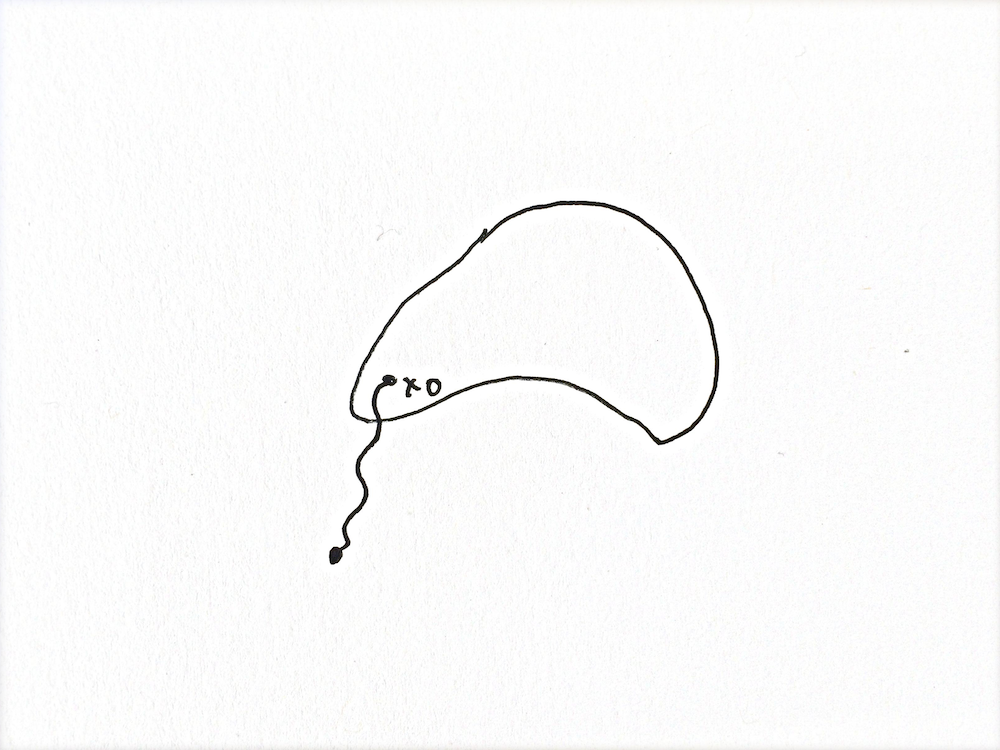
\includegraphics{pics/whisker.png}}
  \centering
\end{figure}



\begin{example} Consider the map $S^1 \to \ast$ collapsing the sphere to a point. The cofiber of this map is $\ast$, that is, a one-point space. However to form the homotopy cofiber, we must draw a path from each point on $S^1$ to the point $\ast$. Here is where we sweep some more rigor under the rug, and illustrate what we mean by ``in a continuous fashion'' in our characterization of homotopy colimits. When creating our paths from points on $S^1$ to $\ast$, a small change in the choice of point on the circle $S^1$ should correspond to a small change in the path drawn. We shouldn't think of these paths as a loose collection of uncountably many strings, flying everywhere and connecting each point on $S^1$ to $\ast$. Instead, nearby strings should coagulate to form surfaces.

\begin{figure}[H]
  \scalebox{0.2}{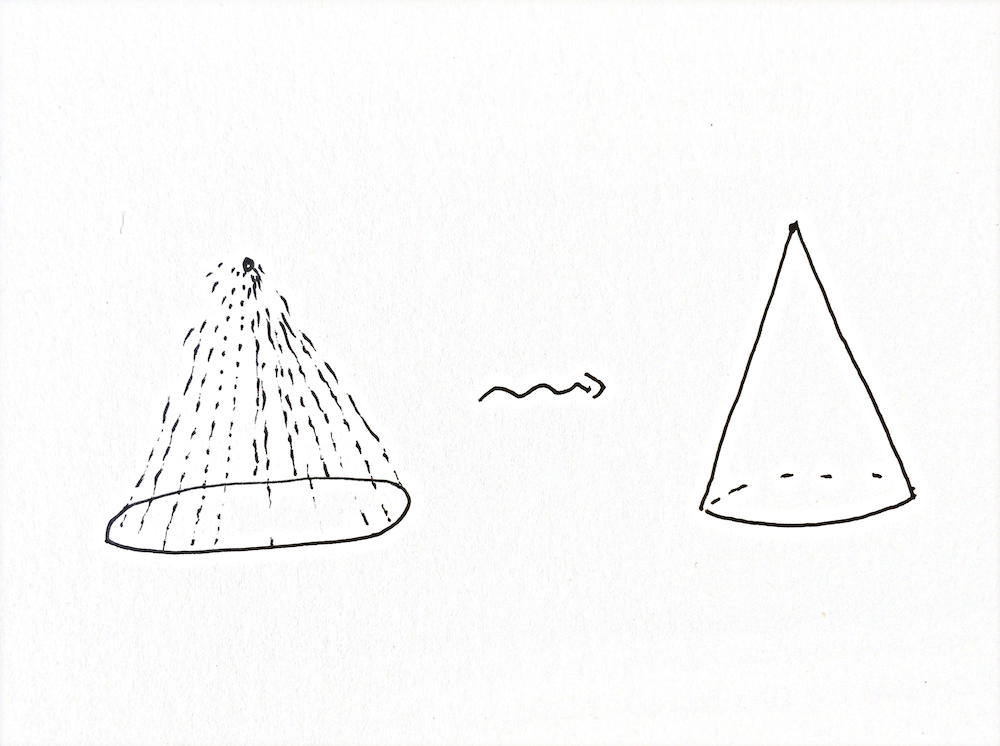
\includegraphics{pics/cone.png}}
  \centering
\end{figure}

If you've followed this rough description, then it would make sense to you that the homotopy cofiber of the map $S^1 \to \ast$ becomes a hollow cone over $S^1$, whose vertex is the point $\ast$. If, on the other hand, this lack of rigor has disgusted you, then the authors understand wholeheartedly and invite you to read \cite{Dugger}.
\end{example}


In the previous examples, the resulting space obtained by taking a homotopy colimit was weakly homotopy equivalent to the original one obtained by taking a colimit. We can ask whether this will always be the case, which the following example (a rephrased version of Example 2.1 in \cite{Dugger}) illustrates.


\begin{example} Consider the diagram $\ast \from S^1 \to \ast$. Its colimit is the pushout $\ast \amalg_{S^1} \ast \cong \ast$, which is just a one-point space. On the other hand, its homotopy colimit can be constructed via the previous example. By gluing $S^1$ to each point $\ast$, we obtain two hollow cones which are identified together along their bases. That is, we obtain a 2-sphere $S^2$. Note that $S^2 \not \simeq \ast$!
\end{example}

This is an example of a general phenomena; for a diagram $D: I \to \Top$, it is often the case that $\colim(D) \not\simeq \hocolim(D)$.


\begin{remark} In the previous section we have said that a homotopy colimit ``is'' a certain space. The reader should be advised that homotopy colimits are only defined up to weak equivalence. This turns out to be both a blessing and a curse, in that we fail to obtain a well-defined construction in the topological category, however the ambiguity allows homotopy colimits to satisfy a property that colimits fail to satisfy: \textit{homotopy invariance.} We will make this precise.
\end{remark}

\subsection{Homotopy Invariance}

\begin{definition} A \textit{weak homotopy equivalence of diagrams} is a natural transformation $D \Rightarrow D'$ (occasionally denoted $D \simeq D'$) between two diagrams $D,D' : I \to \Top$ whose components are weak homotopy equivalences.
\end{definition}

\begin{example}\label{ex:we-of-diagrams} Let our index category be $I = \bullet \from \bullet \to \bullet$, and let $D(I) = \left(D^{n+1} \hookfrom S^n \hookto D^{n+1}\right)$, and $D'(I) = \left(\ast \from S^n \to \ast \right)$. Then there is a weak homotopy equivalence of diagrams $D \Rightarrow D'$ whose components are the identity map on $S^n$ and the contraction $D^{n+1} \xto{\sim} \ast$ on the disks.
\end{example}

\begin{remark} Colimits fail to satisfy \textit{homotopy invariance}. That is, for a weak homotopy equivalence of diagrams $D\simeq D'$, we may have that $\colim(D) \not\simeq \colim(D')$.
\end{remark}

\begin{exercise} See in Example \ref{ex:we-of-diagrams} that $\colim(D) = S^{n+1}$ but $\colim(D') = \ast$.
\end{exercise}

\begin{theorem} Homotopy colimits satisfy homotopy invariance. That is, for $D\simeq D'$, one always has that
\begin{align*}
    \hocolim(D) \simeq \hocolim(D').
\end{align*}
\end{theorem}

\begin{corollary} Given any diagram, we may replace maps and objects in the diagram by weakly equivalent ones and obtain the same homotopy colimit.
\end{corollary}


\subsection{Homotopy colimits coinciding with colimits}

There are many deep questions to ask about homotopy colimits, but perhaps the first one that we might be curious about is when homotopy colimits and colimits coincide. This question is non-trivial to answer, and as always we defer to \cite{Dugger} for a full treatment. However we will give one example, which is a stronger condition on a diagram than one needs in general, but will suit our examples:

\begin{proposition} If a diagram $D: I \to \Top$ has the property that all of its maps are cofibrations, then $\colim(D) \simeq \hocolim(D)$.
\end{proposition}

In particular, if the maps are inclusions of subspaces which form a relative CW complex, they are cofibrations.

This fact, combined with homotopy invariance of homotopy colimits, will allow us to provide a characterization of a lot of phenomena occurring in algebraic topology in terms of homotopy colimits.

\begin{example} We have that $\Sigma X = \hocolim(\ast \from X \to \ast)$.
\end{example}
\begin{proof} Let $CX$ denote the cone over $X$, and note that $CX \simeq \ast$ is contractible. Then since the inclusion $X \hookto CX$ is a relative CW complex, one has
\begin{align*}
    \Sigma X &= \colim \left( \begin{tikzcd}[ampersand replacement=\&] X\rar[hook]\dar[hook] \& CX \\ CX \& \end{tikzcd} \right) = \hocolim \left( \begin{tikzcd}[ampersand replacement=\&] X\rar[hook]\dar[hook] \& CX \\ CX \& \end{tikzcd} \right) \\
    &=\hocolim \left( \begin{tikzcd}[ampersand replacement=\&] X\rar[hook]\dar[hook] \& \ast \\ \ast \& \end{tikzcd} \right).
\end{align*}
\end{proof}

\begin{example} Let $\phi: S^n \to X_n$ be the attaching map for an $(n+1)$-cell, and let $X_{n+1}$ be the space obtained by attaching this cell. Then
\begin{align*}
    X_{n+1} = \hocofib\left(S^n \xto{\phi} X_n\right).
\end{align*}
\end{example}
\begin{proof} Again we apply the previous proposition and homotopy invariance of homotopy colimits. We have that
\begin{align*}
    X_{n+1} &= \colim \left( \begin{tikzcd}[ampersand replacement=\&] S^n\rar[hook,"\phi" above]\dar[hook] \& X_n \\ D^{n+1} \& \end{tikzcd} \right) = \hocolim \left( \begin{tikzcd}[ampersand replacement=\&] S^n\rar[hook,"\phi" above]\dar[hook] \& X_n \\ D^{n+1} \& \end{tikzcd} \right) \\
    &=\hocolim \left( \begin{tikzcd}[ampersand replacement=\&] S^n\rar[hook,"\phi" above]\dar[hook] \& X_n \\ \ast \& \end{tikzcd} \right) = \hocofib(\phi).
\end{align*}
\end{proof}

\begin{example} For a map $f: X\to Y$, the \textit{mapping cylinder}, defined on \cite[p.2]{hatcher} may be thought of as $M_f = \hocolim(X \xto{f} Y)$.
\end{example}


\begin{example} For a map $f: X\to Y$ \textit{mapping cone} $C_f$, defined on \cite[p.13]{hatcher}, is the homotopy cofiber of the map $f$:
\begin{align*}
    C_f = \hocofib(f).
\end{align*}
\end{example}

\begin{example} The \textit{join} of two spaces $X$ and $Y$, defined on \cite[p.9]{hatcher}, is the homotopy pushout $\hocolim(X \from X\times Y \to Y)$.
\end{example}

\begin{example} As a generalization of the previous example, the \textit{double mapping cylinder}, defined on \cite[p.80]{may}, is the homotopy pushout $\hocolim( A \from X \to B)$.
\end{example}

\begin{example} The \textit{mapping telescope}, defined on \cite[p.138]{hatcher}, is the homotopy colimit
\begin{align*}
    \hocolim\left(X_0 \xto{f_0} X_1 \xto{f_1} \cdots \right).
\end{align*}

\end{example}




\begin{theorem} \cite[Theorem~24.9]{chacholski} Homotopy colimits commute.
\end{theorem}

\begin{corollary} On \cite[p.57]{may}, a critical aspect of the cofiber sequence generated by a map $f$ is that there is a weak equivalence (really a homeomorphism) $\Sigma C_f \simeq C(\Sigma f)$. This can be easily remembered by the fact that homotopy colimits commute.
\end{corollary}


